% RHM update, 2026-11-18: what the Random Hierarchy Model is, what the tree tensor network learned on it, and the
% two provable toy grammars run on 2026-11-17 (rhm-forced-synonyms, rhm-crossed-rank, rhm-toy-rerun).
% Build from this directory with: latexmk -pdf -halt-on-error slides.tex
% What to say on each slide is in script.md.
% Figures: figures/make_figures.py redraws them from the saved results (run from the repository root).
% Tensor network diagrams use tensor-network.sty from github.com/mptoolkit/tikz-diagrams (GPL-3), copied here.
\documentclass[aspectratio=169,12pt,t]{beamer}
\usepackage[T1]{fontenc}
\usepackage{lmodern,tgpagella,tgheros}
\usepackage{amsmath,amssymb,graphicx,tikz,booktabs,array}
\usepackage{tensor-network}
\usepackage{pifont}
\newcommand{\yes}{\ding{51}}
\newcommand{\no}{\ding{55}}
\usetikzlibrary{arrows.meta,calc}
\usefonttheme[onlymath]{serif}
\definecolor{ink}{gray}{0.09}
\definecolor{secondary}{gray}{0.33}
\definecolor{aligned}{HTML}{0F4D92}   % figures4papers blue: the tree that matches the grammar
\definecolor{crossed}{HTML}{B64342}   % figures4papers red: the tree that does not
\setbeamercolor{normal text}{fg=ink,bg=white}
\setbeamercolor{structure}{fg=ink}
\setbeamercolor{frametitle}{fg=ink,bg=white}
\setbeamerfont{title}{family=\rmfamily,series=\bfseries}
\setbeamerfont{frametitle}{parent=title,size=\Large}
\setbeamerfont{block title}{family=\rmfamily,series=\bfseries}
\setbeamersize{text margin left=9mm,text margin right=9mm}
\setbeamertemplate{navigation symbols}{}
\setbeamertemplate{headline}{}
\setbeamertemplate{footline}{}
\setbeamertemplate{frametitle}{%
  \vspace*{4mm}\noindent\usebeamerfont{frametitle}\insertframetitle\par}
\setbeamertemplate{itemize item}{\raisebox{0.2ex}{\tiny$\bullet$}}
\setbeamertemplate{enumerate item}{\insertenumlabel.}
\newcommand{\contextline}[1]{{\par\centering\small\color{secondary}#1\par}}
\newcommand{\sym}{\textsf{sym}}
\newcommand{\modg}{\textsf{mod}}
\newcommand{\rd}{\mathrm{read}}
\hypersetup{pdftitle={Tree tensor networks on the Random Hierarchy Model},pdfauthor={}}

% Tensor network pictures: circles are trained cores, dots are data, every edge carries its dimension.
\tnsetup{tensorsize=11pt, xscale=1, yscale=1, outer xsep=0pt, outer ysep=0pt, tensor fill=gray!12}
\tikzset{
  dim/.style={font=\scriptsize, inner sep=1.2pt, text=ink},
  data/.style={circle, fill=ink, inner sep=0pt, minimum size=3.2pt},
  lev/.style={anchor=west, font=\footnotesize, align=left, text=ink, inner sep=0pt},
  levsec/.style={lev, text=secondary}}

\begin{document}

% ---------------------------------------------------------------------------------------------------------------
% The grammar. Source: studies/rhm/grammar.py. Standard configuration v = n = 16, m = 4, s = 2, L = 4.
\begin{frame}{The Random Hierarchy Model}
  \vspace{3mm}
  \begin{columns}[c,onlytextwidth]
    \begin{column}{.60\linewidth}
      \centering
      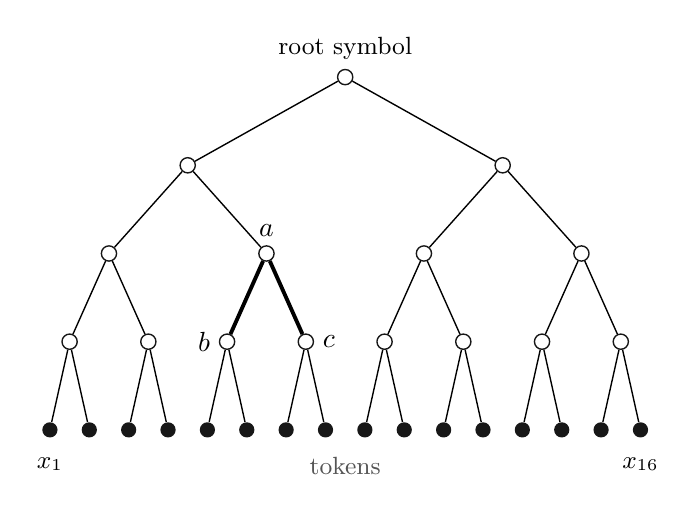
\begin{tikzpicture}[x=0.5cm,y=1.12cm,
          latent/.style={circle,draw=ink,fill=white,inner sep=0pt,minimum size=5.5pt,line width=.5pt},
          token/.style={circle,fill=ink,inner sep=0pt,minimum size=5.5pt}]
        % level l has 2^l nodes; node k of level l sits above the middle of its 2^(4-l) tokens
        \foreach \l/\cnt/\wd in {0/1/16,1/2/8,2/4/4,3/8/2}{
          \foreach \k in {1,...,\cnt}{
            \pgfmathsetmacro{\x}{(\k-0.5)*\wd-0.5}
            \node[latent] (n\l-\k) at (\x,4-\l) {};
          }
        }
        \foreach \k in {1,...,16}{ \node[token] (n4-\k) at (\k-1,0) {}; }
        \foreach \l/\cnt in {0/1,1/2,2/4,3/8}{
          \pgfmathtruncatemacro{\next}{\l+1}
          \foreach \k in {1,...,\cnt}{
            \pgfmathtruncatemacro{\a}{2*\k-1}
            \pgfmathtruncatemacro{\b}{2*\k}
            \draw[line width=.5pt] (n\l-\k) -- (n\next-\a);
            \draw[line width=.5pt] (n\l-\k) -- (n\next-\b);
          }
        }
        % one production, drawn heavier
        \draw[line width=1.4pt] (n2-2) -- (n3-3) (n2-2) -- (n3-4);
        \node[anchor=south,inner sep=3pt] at (n2-2.north) {$a$};
        \node[anchor=east,inner sep=3pt] at (n3-3.west) {$b$};
        \node[anchor=west,inner sep=3pt] at (n3-4.east) {$c$};
        \node[font=\small,anchor=south] at (n0-1.north) {root symbol};
        \node[font=\small,anchor=north] at (0,-0.2) {$x_1$};
        \node[font=\small,anchor=north] at (15,-0.2) {$x_{16}$};
        \node[font=\small,anchor=north,text=secondary] at (7.5,-0.2) {tokens};
      \end{tikzpicture}
    \end{column}
    \begin{column}{.38\linewidth}
      \[ a \;\to\; b\,c \mid d\,e \mid f\,g \mid h\,k \]
      \contextline{$m=4$ synonyms per symbol}
      \vspace{5mm}
      \[
        \begin{aligned}
          \textbf{root:}\quad & x_{1:16} \mapsto \text{root symbol}\\
          \textbf{last:}\quad & x_{1:15} \mapsto x_{16}
        \end{aligned}
      \]
      \vspace{1mm}
      \[ P^* = n\,m^L = 4{,}096 \]
    \end{column}
  \end{columns}
  \vspace{3mm}
  \contextline{$v = n = 16$ symbols per level, depth $L=4$ \qquad Cagnetta et al.\ (2024)}
\end{frame}

% ---------------------------------------------------------------------------------------------------------------
% The model. Source: ctn/tree.py (TreeTN). Parameters n V r + (n - 2) r^3 + O r^2 = 65,536 at V = r = O = 16:
% 16 x 256 (embeddings) + 14 x 4,096 (fusion cores) + 4,096 (root core).
\begin{frame}{The tree tensor network has the grammar's shape}
  \vspace{3mm}
  \centering
  \begin{tikzpicture}[tensornetwork, x=0.54cm, y=0.94cm, line width=0.5pt]
    % leaves: data dot, physical leg of dimension V, embedding A_i
    \foreach \k in {1,...,16}{
      \node[data] (x\k) at (\k-1,0) {};
      \node[atensor] (t0-\k) at (\k-1,0.85) {};
      \draw (x\k) -- (t0-\k) node[dim,midway,right] {$V$};
    }
    % fusion cores, level l = 1..3, then the root core
    \foreach \l/\cnt/\wd in {1/8/2,2/4/4,3/2/8}{
      \foreach \k in {1,...,\cnt}{
        \pgfmathsetmacro{\x}{(\k-0.5)*\wd-0.5}
        \node[atensor] (t\l-\k) at (\x,0.85+\l) {};
      }
    }
    \node[atensor] (C) at (7.5,4.85) {};
    \foreach \l/\cnt in {1/8,2/4,3/2}{
      \pgfmathtruncatemacro{\prev}{\l-1}
      \foreach \k in {1,...,\cnt}{
        \pgfmathtruncatemacro{\a}{2*\k-1}
        \pgfmathtruncatemacro{\b}{2*\k}
        \draw (t\prev-\a) -- (t\l-\k) node[dim,midway,left] {$r$};
        \draw (t\prev-\b) -- (t\l-\k) node[dim,midway,right] {$r$};
      }
    }
    \draw (t3-1) -- (C) node[dim,midway,above left] {$r$};
    \draw (t3-2) -- (C) node[dim,midway,above right] {$r$};
    \draw (C) -- ++(0,0.7) node[dim,midway,right] {$O$} coordinate (out);
    \node[font=\footnotesize,anchor=south,inner sep=2pt] at (out) {logits, $O=16$};
    \node[font=\footnotesize,anchor=north] at (0,-0.15) {$x_1$};
    \node[font=\footnotesize,anchor=north] at (15,-0.15) {$x_{16}$};
    % each level: its tensors, their shape, and the parameter count at V = r = O = 16
    \def\xl{16.6}
    \def\xp{25.6}
    \node[lev] at (\xl,4.85) {$C\in\mathbb{R}^{O\times r\times r}$};
    \node[lev] at (\xl,3.85) {$2\times W\in\mathbb{R}^{r\times r\times r}$};
    \node[lev] at (\xl,2.85) {$4\times W$};
    \node[lev] at (\xl,1.85) {$8\times W$};
    \node[lev] at (\xl,0.85) {$16\times A_i\in\mathbb{R}^{r\times V}$};
    \node[lev] at (\xl,0) {one-hot, $V=16$};
    \foreach \y/\n in {4.85/{4{,}096},3.85/{8{,}192},2.85/{16{,}384},1.85/{32{,}768},0.85/{4{,}096}}{
      \node[levsec,anchor=east] at (\xp,\y) {\n};
    }
    \draw[secondary,line width=0.4pt] (\xp-2.6,0.4) -- (\xp,0.4);
    \node[levsec,anchor=east] at (\xp,0) {65{,}536};
    \node[levsec,anchor=east] at (\xp,5.45) {parameters, $r=16$};
  \end{tikzpicture}

  \vspace{4mm}
  \(z_i = A_i\,e_{x_i}, \qquad
    z_{\text{parent}} = W(z_{\text{left}}, z_{\text{right}}), \qquad
    \text{logits} = C(z_{\mathrm L}, z_{\mathrm R})\)
\end{frame}

% ---------------------------------------------------------------------------------------------------------------
% figures/learning.pdf. Left: rhm-sample-efficiency (results/analysis.json). Right: rhm-controls (results/curves.json).
\begin{frame}{The matching tree learns the RHM near $P^*$}
  \vspace{1mm}
  \centering
  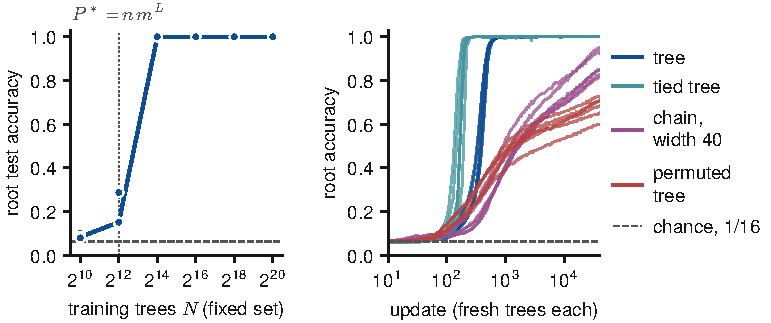
\includegraphics[width=\linewidth,height=.70\paperheight,keepaspectratio]{figures/learning.pdf}\par
  \medskip
  \contextline{root task, three grammars, trees at $r=16$ \qquad 65k parameters (tied tree: 16.6k)}
\end{frame}

% ---------------------------------------------------------------------------------------------------------------
% Numbers: rhm-transfer/README.md, and HANDOFF.md for rhm-ttn-belief-geometry, rhm-ttn-messages, rhm-ttn-masks.
\begin{frame}{Bonds hold the belief, not the grammar's messages}
  \vspace{6mm}
  \centering
  \renewcommand{\arraystretch}{1.7}
  \begin{tabular}{@{}cl@{\qquad}l@{}}
    \yes & lower subtrees transfer & 42 updates frozen, 148 from scratch\\
    \yes & top bonds $\Rightarrow$ Bayes belief & 7 of 8 grammars, $R^2$ 0.85 to 1.00\\
    \no & bond $=$ the grammar's message & 0 of 9 cells, $R^2$ 0.08 to 0.75\\
    \no & merge $=$ the message update & 0 of 9 cells, $R^2$ 0.17 to 0.58\\
    \no & mixed-mask training repairs it & 0 of 12 runs\\
  \end{tabular}

  \vspace{6mm}
  \contextline{a probe test passes at $R^2 \ge 0.8$}
\end{frame}

% ---------------------------------------------------------------------------------------------------------------
% figures/belief_mess3.pdf: hmm-belief-geometry, seed 0, redrawn from results/mess3_<model>_s0/proj_ckpt*.npz.
% Scope: HANDOFF.md (belief batch) and studies/hmm/hmm-belief-geometry/README.md.
\begin{frame}{Mess3: every probe recovers the belief simplex}
  \vspace{1mm}
  \centering
  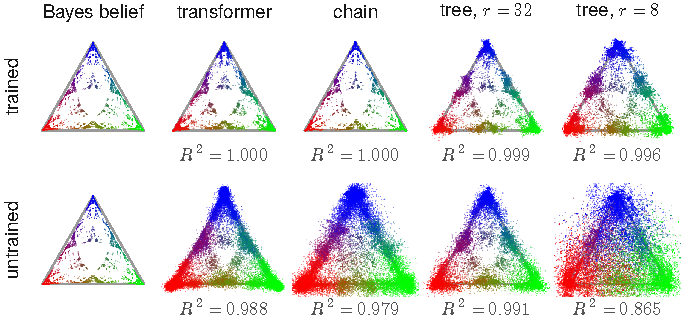
\includegraphics[width=\linewidth,height=.66\paperheight,keepaspectratio]{figures/belief_mess3.pdf}\par
  \medskip
  \contextline{seed 0 \qquad on Mess3 the belief follows from the next-token prediction}
\end{frame}

% ---------------------------------------------------------------------------------------------------------------
% figures/belief_rrxor.pdf: hmm-belief-geometry, seed 0, redrawn from results/rrxor_<model>_s0/proj_ckpt*.npz.
\begin{frame}{RRXOR: belief states, not yet belief geometry}
  \vspace{1mm}
  \centering
  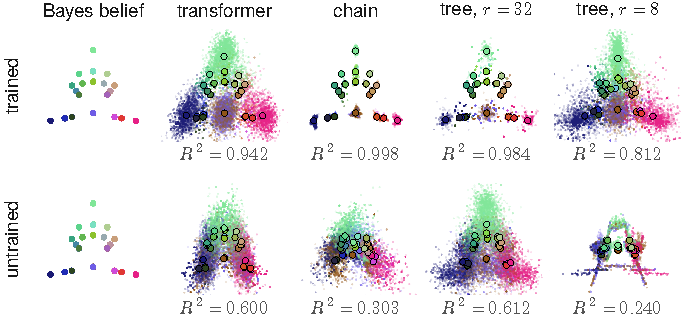
\includegraphics[width=\linewidth,height=.66\paperheight,keepaspectratio]{figures/belief_rrxor.pdf}\par
  \medskip
  \contextline{seed 0 \qquad next-token ceiling 0.47 \qquad random-label control 0.88 to 0.92 (chain)}
\end{frame}

% ---------------------------------------------------------------------------------------------------------------
% figures/factored.pdf: belief-probe-controls/results/factor_product.json (a reanalysis of saved checkpoints).
\begin{frame}{The tensor networks keep marginals, not the joint}
  \vspace{1mm}
  \centering
  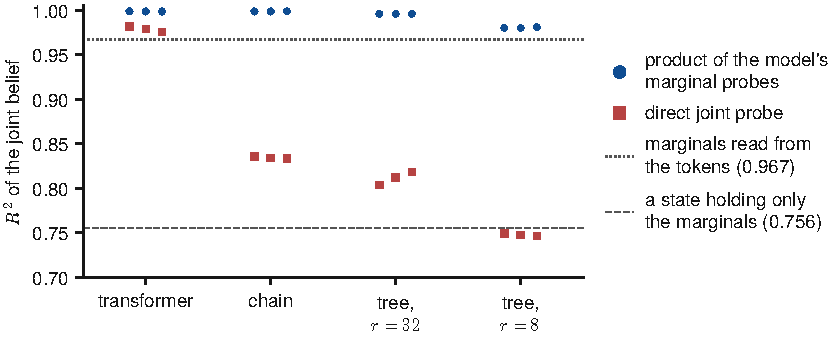
\includegraphics[width=\linewidth,height=.68\paperheight,keepaspectratio]{figures/factored.pdf}\par
  \medskip
  \contextline{two independent 3-state processes, three seeds \qquad tree: first half only}
\end{frame}

% ---------------------------------------------------------------------------------------------------------------
% The toy setting. Source: studies/rhm/toy.py. TreeTN(n=8, V=4, r, O=3); crossed = leaves 2 and 3 swapped.
\begin{frame}{Two 3-symbol grammars with provable optima}
  \vspace{1mm}
  \begin{columns}[c,onlytextwidth]
    \begin{column}{.45\linewidth}
      \renewcommand{\arraystretch}{1.15}
      \begin{tabular}{@{}l@{\quad}l@{}}
        \sym & $0\to12\mid21$\\
        {\footnotesize\color{secondary}every level} & $1\to02\mid20$\\
             & $2\to01\mid10$\\[2.5mm]
        \modg & $0\to12\mid21$\\
        {\footnotesize\color{secondary}bottom level} & $1\to02\mid22$\\
              & $2\to01\mid11$
      \end{tabular}
      \[
        P(x_5 = y \mid x_{1:4}) =
        \begin{cases} 1/4 & y = A\\ 3/8 & y\neq A\end{cases}
      \]
    \end{column}
    \begin{column}{.53\linewidth}
      \centering
      \begin{tikzpicture}[tensornetwork, x=0.8cm, y=0.9cm, line width=0.5pt]
        \foreach \k in {1,...,8}{
          \node[data] (x\k) at (\k-1,0) {};
          \node[atensor] (t0-\k) at (\k-1,0.85) {};
          \draw (x\k) -- (t0-\k) node[dim,midway,right] {4};
        }
        \foreach \l/\cnt/\wd in {1/4/2,2/2/4}{
          \foreach \k in {1,...,\cnt}{
            \pgfmathsetmacro{\x}{(\k-0.5)*\wd-0.5}
            \node[atensor] (t\l-\k) at (\x,0.85+\l) {};
          }
        }
        \node[atensor] (C) at (3.5,3.85) {};
        \foreach \l/\cnt in {1/4,2/2}{
          \pgfmathtruncatemacro{\prev}{\l-1}
          \foreach \k in {1,...,\cnt}{
            \pgfmathtruncatemacro{\a}{2*\k-1}
            \pgfmathtruncatemacro{\b}{2*\k}
            \draw (t\prev-\a) -- (t\l-\k) node[dim,midway,left] {$r$};
            \draw (t\prev-\b) -- (t\l-\k) node[dim,midway,right] {$r$};
          }
        }
        \draw (t2-1) -- (C) node[dim,midway,above left] {$r$};
        \draw (t2-2) -- (C) node[dim,midway,above right] {$r$};
        \draw (C) -- ++(0,0.7) node[dim,midway,right] {3} coordinate (out);
        \node[font=\footnotesize,anchor=south,inner sep=2pt] at (out) {logits for $x_5$};
        \foreach \k in {1,...,4}{ \node[font=\footnotesize,anchor=north] at (\k-1,-0.12) {$x_\k$}; }
        \node[font=\footnotesize,anchor=north,text=secondary] at (5.5,-0.12) {mask};
        % the crossed pairing swaps the inputs of leaves 2 and 3
        \draw[crossed,<->,>=Stealth,line width=0.7pt] (1,-0.66) to[bend right=50] (2,-0.66);
        \node[font=\footnotesize,text=crossed,anchor=west] at (2.3,-0.88) {crossed};
      \end{tikzpicture}
    \end{column}
  \end{columns}
  \vspace{2mm}
  \contextline{$A$: the symbol above $x_{1:4}$ \qquad $r = 1,\dots,6$ \qquad leg: 3 symbols and a mask}
\end{frame}

% ---------------------------------------------------------------------------------------------------------------
% Theory of rhm-forced-synonyms (NOTE.md, Part 1). Every statement here is proved for exact width-2 trees on sym.
\begin{frame}{At $r=2$ an exact tree has no room for the synonym}
  \vspace{4mm}
  \centering
  \renewcommand{\arraystretch}{1.5}
  \begin{tabular}{@{}l@{\qquad\quad}l@{}}
    $h_{\mathrm L} = a_b,\quad h_{\mathrm R} = c_{c}$ & synonyms share one code\\
    $W(a_b, c_{c}) = p_{\overline{bc}}\quad (b\neq c)$ & codes compose as the grammar does\\
    $W(a_b, c_b) \neq 0$ & forbidden pairs respond
  \end{tabular}

  \vspace{6mm}
  With $a_0 = x\,a_1 + y\,a_2$, the response to $(b,b)$ relative to a valid pair is
  \[
    \rho_0 = \sqrt{x^2+y^2-xy},\qquad
    \rho_1 = \frac{\sqrt{1+y+y^2}}{|x|},\qquad
    \rho_2 = \frac{\sqrt{1+x+x^2}}{|y|}
  \]
  \[ \rho_b\,\rho_{b'} \ge \tfrac34 \]
  \vspace{1mm}
  \contextline{proved for every exact $r=2$ tree on \sym; message passing would give $\rho = 0$}
\end{frame}

% ---------------------------------------------------------------------------------------------------------------
% figures/forbidden.pdf, from rhm-forced-synonyms/results/runs.json. Numbers: rhm-forced-synonyms/README.md.
\begin{frame}{Training follows the formulas and never finds 0}
  \vspace{1mm}
  \centering
  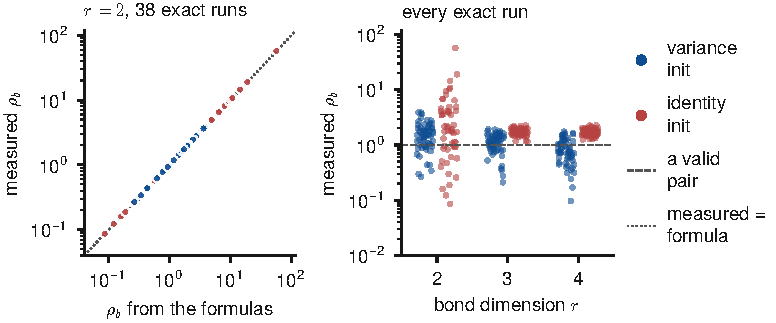
\includegraphics[width=\linewidth,height=.70\paperheight,keepaspectratio]{figures/forbidden.pdf}\par
  \medskip
  \contextline{\sym, 20 seeds $\times$ 2 inits per width \qquad message passing: $\rho_b = 0$}
\end{frame}

% ---------------------------------------------------------------------------------------------------------------
% Theory of rhm-crossed-rank (NOTE.md). The 4 x 4 block is in units of log(2/3)/3, outputs y = 0, 1 of each context.
\begin{frame}{Every bond bounds a rank}
  \vspace{1mm}
  \[
    \ell_y(x) = \sum_{k=1}^{r} u_k(x_S)\,v_k(x_{\bar S},y)
    \quad\Longrightarrow\quad
    r \;\ge\; \max_{\text{bonds}}\ \max_{\text{legal blocks}}\ \operatorname{rank} F\big|_{\text{block}}
  \]
  \vspace{-1mm}
  \begin{columns}[c,onlytextwidth]
    \begin{column}{.44\linewidth}
      \centering
      \small
      \renewcommand{\arraystretch}{1.0}
      \begin{tabular}{@{}ccc@{}}
        \toprule
        $x_1x_3$ & $x_2x_4=12$ & $x_2x_4=21$\\
        \midrule
        00 & $A=0$ & $A=0$\\
        01 & $A=1$ & $A=0$\\
        02 & $A=0$ & $A=2$\\
        10 & $A=0$ & $A=1$\\
        \bottomrule
      \end{tabular}
    \end{column}
    \begin{column}{.54\linewidth}
      \[
        F\big|_{\text{block}} \propto \begin{pmatrix} 2&-1&2&-1\\ -1&2&2&-1\\ 2&-1&-1&-1\\ 2&-1&-1&2 \end{pmatrix},
        \quad \det \neq 0
      \]
    \end{column}
  \end{columns}
  \vspace{5mm}
  \centering
  \begin{tabular}{@{}l@{\qquad}l@{\qquad\qquad}l@{}}
    \modg: & {\color{aligned}aligned $r\ge3$}, \ {\color{crossed}crossed $r\ge4$} & \sym: \ $r\ge2$ for both
  \end{tabular}
\end{frame}

% ---------------------------------------------------------------------------------------------------------------
% figures/capacity.pdf, from rhm-crossed-rank/results/{runs,summary}.json. Numbers: rhm-crossed-rank/README.md.
\begin{frame}{Training is exact only where the bounds allow}
  \vspace{1mm}
  \centering
  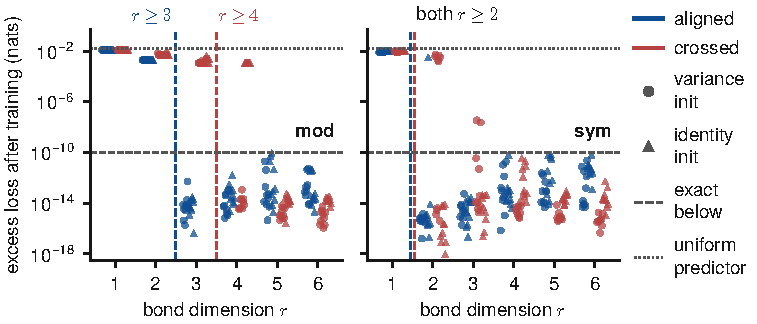
\includegraphics[width=\linewidth,height=.70\paperheight,keepaspectratio]{figures/capacity.pdf}\par
  \medskip
  \contextline{20 runs per cell \qquad dashed colored lines: the proved lower bounds}
\end{frame}

% ---------------------------------------------------------------------------------------------------------------
% Learning-rate arm of rhm-crossed-rank (README.md and NOTE.md); the post-hoc check is results/posthoc.txt.
\begin{frame}{The crossed tree is harder to find at its bound}
  \vspace{2mm}
  \footnotesize
  \centering
  \renewcommand{\arraystretch}{1.1}
  \begin{tabular}{@{}ll*{4}{>{\centering\arraybackslash}p{17mm}}@{}}
    \toprule
    & & \multicolumn{4}{c}{exact runs of 10 seeds, by learning rate}\\
    \cmidrule(l){3-6}
    & init & $10^{-3}$ & $3\times10^{-3}$ & $10^{-2}$ & $3\times10^{-2}$\\
    \midrule
    \sym{} {\color{aligned}aligned}, $r=2$ & variance & 10 & 10 & 10 & 10\\
                                           & identity & 4 & 9 & 10 & 10\\
    \addlinespace
    \sym{} {\color{crossed}crossed}, $r=2$ & variance & 5 & 4 & 4 & 5\\
                                           & identity & 9 & 10 & 10 & 9\\
    \addlinespace
    \modg{} {\color{aligned}aligned}, $r=3$ & variance & 10 & 10 & 10 & 9\\
                                            & identity & 10 & 10 & 10 & 10\\
    \addlinespace
    \modg{} {\color{crossed}crossed}, $r=4$ & variance & 10 & 10 & 10 & 10\\
                                            & identity & 0 & 0 & 0 & 7\\
    \bottomrule
  \end{tabular}

  \vspace{4mm}
  \contextline{the ten \modg{} misses at $3\times10^{-3}$ end on the $r=3$ floor, $1.149171\times10^{-3}$ nats}
\end{frame}

% ---------------------------------------------------------------------------------------------------------------
% Rerun: rhm-toy-rerun/README.md. Follow-ups: the lists at the end of the two NOTE.md files and HANDOFF.md.
\begin{frame}{Which follow-up first?}
  \vspace{8mm}
  \begin{enumerate}
    \setlength{\itemsep}{7mm}
    \item The 40 width-2 seeds under plain gradient descent
    \item A closed-form $r=4$ crossed tree for \modg
    \item The same rank bounds on the larger RHM grammars
  \end{enumerate}
  \vspace{9mm}
  \contextline{rerun on a second machine: every verdict equal, all 880 run files identical apart from wall-clock time}
\end{frame}

\end{document}
